% !TEX root = main_min_disc_dist.tex
\subsection{Pursuit-Evasion Game}

We now consider the pursuit-evasion game described in \cite{Mitchell2005}. In the game player I (the control) tries to avoid being captured by player II (the disturbance) on a two dimensional plane. Each player is modeled as a simple kinematic point object with planar position and heading, fixed linear velocity and controllable angular velocity. Taking player I to be at the origin the states $(x_1, x_2, x_3)$ are the relative position and heading of player II and the dynamics are

\begin{equation}
\begin{split}
&\dot{x_1}= -v_u+v_d \cos x_3 + ux_2\\ 
&\dot{x_2}= v_d \sin x_3 - ux_1\\ 
&\dot{x_3}= d-u
\end{split}
\end{equation}

The state space is over the domain $[-6,20] \times [-10,10] \times [0,2\pi[$ with $\U=[-u_{max},u_{max}]$ and $\D=[-d_{max}, d_{max}]$. 

Player I is considered captured when the relative distance (in position) between both players is less than $R>0$, thus the target set is given by

\begin{equation}
\T= \{x| x_1^{2}+x_2^2 < R\}
\end{equation}


We first compute the value functions for the MR and MDR on a $41 \times 41 \times 41$ grid, and setting the model parameters to $v_u=v_d=5$, $u_{max}=d_{max}=1$, and $R=5$. This will be referred to as model 1. A visualization of the zero sub-level set for both $V(x)$ and $Z(x)$ for $\lambda=0.001$ is shown in Fig~\ref{fig:air3D}.


\begin{figure}
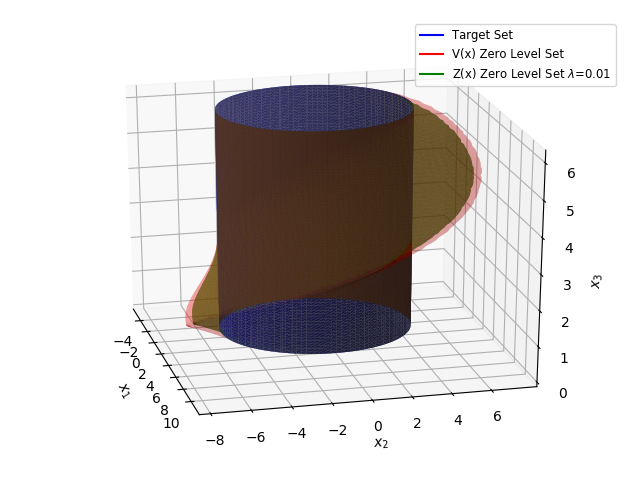
\includegraphics[trim= 2.5cm 0cm 0cm 0.5cm, clip=true,scale=0.65]{air_3D.png}
\caption{The target set $\mathcal{T}$ is the blue cylinder. The zero sub-level sets of $V$ and $Z$ are in red and blue, respectively. The discount rate is $\lambda=0.01$.}
\label{fig:air3D}
\end{figure}

In the first experiment we compare a multigrid approach{} to value iteration. For the multigrid approach we also need to run value iteration on a coarse grid, which we construct to have half the resolution per dimension of the nominal grid, e.g. if the nominal grid has $41^3$ nodes then the coarse grid has $21^3$ nodes. The results are shown in Table~\ref{tab:multigrid}. The multigrid approach outperforms value iteration, especially as the number of nodes increases.

\begin{table}
\centering
\caption{Value Iteration (VI) vs. Multigrid (M)}
\label{tab:multigrid}
\begin{tabular}{|c| c| c| c| }
\hline
\# nodes &  VI coarse & VI & M \\ \hline
$41^3$ &$1.299$ &$15.789$  & $12.190$ \\ \hline
$81^3$ &$16.906$&$256.232$  & $174.385$ \\ \hline
\end{tabular}
\end{table}

We now construct two other models by tweaking model 1: setting $u_{max}=1.5$ produces model 2 and setting $d_{max}=1.5$ produces model 3. In the final experiment we look at the impact of initializing value iteration with a solution from a similar model. As alluded to in Section \ref{sec:learn} this can be beneficial when the model is being iteratively learned. In this context we have just ``learned" that the evader/pursuer is more maneuverable (model 2/model 3). We compute both value functions with and without initializing with the solution for model 1. We refer to this initialization as a \emph{warm start}. The results are shown in Table~\ref{tab:pursuit_evasion}.

\begin{table}
\centering
\caption{Pursuit-Evasion for various models ($M$) with and without warm start ($W$)}
\label{tab:pursuit_evasion}
\begin{tabular}{|c| c| c| c| c|c|}
\hline
\# nodes & $M_1$ & $M_2$ & $M_2$  $W$ & $M_3$ & $M_3$  $W$\\ \hline
$41^3$ & $20.84$ & $18.32$ & $12.66$ & $14.32$ & $8.89$ \\ \hline
$81^3$ & $339.66$ & $339.66$ & $224.29$ & $267.81$ & $166.95$ \\ \hline
\end{tabular}
\end{table}